%% -*- coding:utf-8 -*-

\section{局部性}
%\section{Locality}
\label{Abschnitt-Diskussion-Lokalitaet}\label{sec-locality}

就\isce[|(]{局部性}{locality}信息局部可及这个问题,本书中论及的不同理论有不同的处理方式。在大部分理论中,都尽力让短语的内部结构对于邻接或者更高的中心语不可及,也就是说(\mex{1})中的glaubt(相信)可以选择一个句子论元但是不能选择句子内部的论元。
%The\is{locality|(} question of local accessibility of information has been treated in various ways by the theories
%discussed in this book. In the majority of theories, one tries to make information about the inner workings of phrases inaccessible
%for adjacent or higher heads, that is, \emph{glaubt} `believe' in (\mex{1}) selects a sentential argument but it cannot ``look
%inside'' this sentential argument.
\eal
\ex 
\gll Karl glaubt, dass morgen seine Schwester kommt.\\
	 Karl 相信 \textsc{comp} 明天 他的 姐姐 来\\
\mytrans{Karl相信他的姐姐明天将会来。}
%\gll Karl glaubt, dass morgen seine Schwester kommt.\\
%	 Karl believes that tomorrow his sister comes\\
%\mytrans{Karl believes that his sister is coming tomorrow.}
\ex 
\gll Karl glaubt, dass seine Schwester morgen kommt.\\
	 Karl 相信 \textsc{comp} 他的 姐姐 明天 来\\
%\gll Karl glaubt, dass seine Schwester morgen kommt.\\
%	 Karl believes that his sister tomorrow comes\\
\mytrans{Karl相信他的姐姐明天将会来。}
\zl
所以,例如glauben不能确保动词的主语以辅音开头或者标句词必须与一个以附加语开头的动词性投射组合。在\ref{Abschnitt-Kopf}中,我们看到根据成分的分布而不是其内部结构对其进行分类是一种很好的做法。如果我们讲到NP框,那么这个NP框里具体包含什么并不重要。唯一重要的是一个给定中心语要与一个带有特定格标记的NP组合。这就叫做选择的局部性。
%Thus for example, \emph{glauben} cannot enforce that the subject of the verb has to begin with a consonant or that the complementizer
%has to be combined with a verbal projection starting with an adjunct.
%In Section~\ref{Abschnitt-Kopf}, we saw that it is a good idea to classify constituents in terms of their distribution and
%independent of their internal structure. If we are  talking about an NP box, then it is not important what this NP box actually
%contains. It is only of importance that a given head wants to be combined with an NP with a
%particular case marking. This is called \emph{locality of selection}.

很多语言学理论都试图实现选择的局部性。使用局部性最简单的形式就是第\ref{Kapitel-PSG}章讨论的短语结构语法所使用的形式。在第\pageref{ditrans-schema}页规则 (\ref{ditrans-schema})⸺这里重复写成(\mex{1})⸺规定一个双及物动词可以与三个名词短语组合,每一个名词短语都带有一个相关格:
%Various linguistic theories have tried to implement locality of selection. The simplest form of this implementation is shown by
%phrase structure grammars of the kind discussed in Chapter~\ref{Kapitel-PSG}. The rule in (\ref{ditrans-schema}) on
%page~\pageref{ditrans-schema}, repeated here as (\mex{1}), states that a ditransitive verb can occur with three noun phrases, each
%with the relevant case:
\ea
\begin{tabular}[t]{@{}l@{ }l@{ }l}
S  & $\to$ & NP({Per1},{Num1},{nom}) \\
   &       & NP(Per2,Num2,{dat})\\
   &       & NP(Per3,Num3,{acc})\\
   &       & V({Per1},{Num1},ditransitive)\\
\end{tabular}
\z
例如,因为NP没有内部结构,所以动词不能要求NP内部有一个关系小句。NP的内部属性对于外部不可见。但是,我们在第\ref{Kapitel-PSG}章看到,短语的一些属性必须对于外部可见。这就是写在框自身上的信息。对于名词短语,至少需要人称、数和格信息以便能说明它们与中心语的关系。在德语中,性的取值也很重要,因为副词短语,像einer nach dem anderen(一个接一个)必须与它所指称的名词的性\isce{性}{gender}是一致的(见第\pageref{Beispiel-einer-nach-dem-anderen}页的例(\ref{Beispiel-einer-nach-dem-anderen}))。除此之外,名词短语的长度信息也是必需的,用于确定它们在句子中的顺序。重的成分通常出现在较轻的成分之后,并经常会外置(参见Behaghel提出的“成分上升率”(Gesetz der wachsenden Glieder)\isce{成分上升率}{Gesetz der wachsenden Glieder}(\citeyear[\page 139]{Behaghel09};\citeyear[\page 86]{Behaghel30})。 
%Since the symbols for NPs do not have any further internal structure, the verb cannot require that there has to be a relative
%clause in an NP, for example. The internal properties of the NP are not visible to the outside.
%We have already seen in the discussion in Chapter~\ref{Kapitel-PSG}, however, that certain properties of phrases have to be outwardly
%visible. This was the information that was written on the boxes themselves. For noun phrases, at least information about
%person, number and case are required in order to correctly capture their relation to a head.
%The gender value is important in German as well, since adverbial phrases such as \emph{einer nach
%  dem anderen} `one after the other' have to agree in gender\is{gender} with the noun they refer to
%(see example (\ref{Beispiel-einer-nach-dem-anderen}) on
%page~\pageref{Beispiel-einer-nach-dem-anderen}). Apart from that, information about the length of
%the noun phrases is required, in order to determine their order in a clause. Heavy constituents are normally ordered after lighter ones, and are also often
%extraposed (cf.\ Behaghel's \textit{Gesetz der wachsenden Glieder}\is{Gesetz der wachsenden Glieder} `Law of increasing constituents' (\citeyear[\page
%139]{Behaghel09}; \citeyear[\page 86]{Behaghel30})). 

力求尽可能严格地遵守局域性的理论必须创立这样的机制,即允许成分只能获得解释成分分布所需的信息。这一点通常通过向短语的父结点投射一定属性来完成。在\xbartc 中,中心语的词性信息会上传到最大投射上:例如,如果中心语是一个N,那么最大投射就是一个NP。在GPSG、HPSG和CxG的部分变体中,都有中心语特征原则(Head Feature Principles)用于特征投射。中心语特征原则确保一整组特征,所谓的中心语特征,显示在中心语的最大投射中。另外,任意一个理论都能表示以下现象:一个成分可以缺少一部分并且这一部分可以通过长距离依存在句子的另外一个位置实现。正如前面在第\pageref{page-Irish-complementizers}页所讨论的那样,存在一些语言其标句词的屈折取决于其补足语是否丢失成分。这意味着这一属性必须以某种方式可及。在GPSG、HPSG和CxG的一些变体中,存在另外的特征集合出现在长距离依存填充语、空位之间的任意一个结点上。在LFG中,用f-结构来表示。利用功能不确定性(Functiional Uncertainty),我们在f-结构\isce{f-结构}{f-structure}中可以找到特定成分在什么位置丢失。在\gbtc 中,移位是循环\iscesub{循环}{cycle}{转换}{transformational}进行的,也就是说,一个成分移动到一个CP的限定语,然后从那里可以移动到下一个最高的CP。在\gbtc 中,中心语可以看到论元的内部,至少可以看到限定语位置的成分。如果标句词能达到相关的限定语位置,那么就可以决定是否有成分从嵌套短语中丢失。在\gbtc 中,也可以分析不定构式中的格指派问题,在这种构式中,格指派动词支配被嵌套短语并且为\mbox{SpecIP}中的成分指派格。图\ref{Abbildung-ECM}显示了来自于 \citew[\page 170]{Haegeman94a-u}的相关结构。
%Theories that strive to be as restrictive as possible with respect to locality therefore have to develop mechanisms that allow one to only
%access information that is required to explain the distribution of constituents.
%This is often achieved by projecting certain properties to the mother node of a phrase. In \xbart, the part of speech a head belongs to is
%passed up to the maximal projection: if the head is an N, for example, then the maximal projection is an NP. In GPSG, HPSG and variants
%of CxG, there are Head Feature Principles responsible for the projection of features. Head Feature Principles ensure that an entire group of
%features, so-called head features, are present on the maximal projection of a head.
%Furthermore, every theory has to be capable of representing the fact that a constituent can lack one of its parts and this part is then realized via a long-distance
%dependency in another position in the clause.
%As previously discussed on page~\pageref{page-Irish-complementizers}, there are languages in which complementizers inflect depending on whether their
%complement is missing a constituent or not. This means that this property must be somehow accessible. In GPSG, HPSG and variants of CxG, there are additional
%groups of features that are present at every node between a filler and a gap in a long-distance dependency.
%In LFG, there is f-structure\is{f-structure} instead. Using Functional Uncertainty, one can look for the position in the f-structure where a particular
%constituent is missing. In \gbt, movement proceeds cyclically\is{cycle!transformational}, that is, an element is moved into the specifier of CP and can
%be moved from there into the next highest CP. It is assumed in \gbt that heads can look inside their arguments, at least they can see the elements in the
%specifier position. If complementizers can access the relevant specifier positions, then they can
%determine whether something is missing from an embedded phrase or not. In \gbt, there was also an analysis of case
%assignment in infinitive constructions in which the case-assigning verb governs into the embedded
%phrase and assigns case to the element in \mbox{SpecIP}. Figure~\ref{Abbildung-ECM} shows the
%relevant structure taken from  \citew[\page 170]{Haegeman94a-u}.
\begin{figure}
\centering
\scalebox{.98}{%
\begin{forest}
sm edges
[IP
	[NP
		[John;John]]
	[I$'$
		[I
			[-s;-\textsc{3sg}]]
		[VP
			[V$'$
				[V
					[believe;相信]]
				[IP
					[NP
						[him;他]]
					[I$'$
						[I
							[to;\textsc{inf}]]
						[VP
							[V$'$
								[V
									[be;\textsc{cop}]]
								[NP
									[a liar;一 \, 骗子,roof]]]]]]]]]]
\end{forest}
}
\caption{\label{Abbildung-ECM}带有例外格标记的AcI构式的分析}
%\caption{\label{Abbildung-ECM}Analysis of the AcI construction with \emph{Exceptional Case Marking}}
\end{figure}%
因为格指派原则(Case Principle)是以这一原则定义的,所以只有定式I可以给主语指派格(参见第\pageref{Kasusprinzip-GB}页),him并没有从I获得格指派。相反,他认为动词believe给内嵌的不定式主语指派了格。
%Since the Case Principle is formulated in such a way that only finite I can assign case to the subject
%(cf.\ page~\pageref{Kasusprinzip-GB}), \emph{him} does not receive case from I. Instead, it is assumed that
%the verb \emph{believe} assigns case to the subject of the embedded infinitive.

可以跨越短语边界指派格的动词叫做ECM动词,其中,ECM表示例外格标记(Exceptional Case Marking,简称ECM)\isce{例外格标记(ECM)}{Exceptional Case Marking (ECM)}。正如名称所示,这种向短语中进行格指派被看作是一种例外。在这一理论的最新版本中(\egc \citealp[\page 120--123]{Kratzer96a}),所有格都可以指派到限定语位置。例如,图\vref{Abbildung-Kratzer}的Voice\iscesubsub{范畴}{category}{功能}{functional}{态}{Voice}中心语给VP限定语的DP指派了一个受格。
%Verbs that can assign case across phrase boundaries are referred to as ECM verbs, where ECM stands for
%\emph{Exceptional Case Marking}\is{Exceptional Case Marking (ECM)}. As the name suggests, this instance of case assignment into a phrase was viewed as an
%exception. In newer versions of the theory (\eg \citealp[\page 120--123]{Kratzer96a}), all case assignment
%is to specifier positions. For example, the Voice\is{category!functional!Voice} head in Figure~\vref{Abbildung-Kratzer} assigns
%accusative to the DP in the specifier of VP.
\begin{figure}
\centering
\begin{forest}
sm edges
[VoiceP
	[DP
		[Mittie;Mittie]]
	[Voice$'$
		[Voice
			[agent;施事]]
		[VP
			[DP
				[the dog;\textsc{da} 狗,roof]]
			[V$'$
				[V
					[feed;喂]]]]]]
\end{forest}
\caption{\label{Abbildung-Kratzer}根据Kratzer的带及物动词的结构分析}
%\caption{\label{Abbildung-Kratzer}Analysis of structures with a transitive verb following Kratzer}
\end{figure}%
因为Voice中心语约束VP中的成分,在该理论中给普通宾语进行格指派也是例外格指派。这一点在Adger版本的最简方案中也是如此,见第\ref{chap-mp}章的讨论。 \citet{Adger2010a}声称他的理论比LFG和HPSG更加严格,因为在他的理论中只能选择单个特征,但是在LFG和HPSG中还可以选择特征束。但是,这类局部约束的强度就被一致\isce{一致}{Agree}操作削弱了,该操作允许非局部特征核查。在Kratzer的方案中,格只能借助\littlevc 来局部地指派给VP内部的宾语(参见\ref{sec-case-mp})。
%Since the Voice head governs into the VP, case assignment to a run-of-the-mill object in this theory
%is an instance of exceptional case assignment as well. The same is true in Adger's version of
%Minimalism, which was discussed in Chapter~\ref{chap-mp}:  \citet{Adger2010a} argues that
%his theory is more restrictive than LFG or HPSG since it is only one feature that can be selected by
%a head, whereas in LFG and HPSG complex feature bundles are selected. However, the strength of
%this kind of locality constraint is weakened by the operation Agree\is{Agree}, which allows for
%nonlocal feature checking. As in Kratzer's proposal, case is assigned nonlocally by \littlev to
%the object inside the VP (see Section~\ref{sec-case-mp}). 

Adger讨论depend这一类动词的PP论元并且注意到这些动词需要特定的PPs,即PP中的介词形式必须是可选的。虽然在依存语法中这很容易做到,在该理论中介词可以直接被选择;在HPSG等理论中对应信息会被投射然后在PP结点上被选择。但是,这要求支配动词能决定被选择成分的至少两个属性:其词类以及介词的形式。这一点在Adger的系统中不可能实现,他将这一问题留待以后研究。当然,可能假设一个onP(包含“on”范畴的介词on的投射)。最简方案中也提出过类似的方法(见\ref{sec-functional-projections-minimalism}的功能投射),但是这一方法很明显没有反映所有介词短语有共性这一现象,这些共性无法反映在使用词特定原子范畴的系统中。
%Adger discusses PP arguments of verbs like \emph{depend} and notes that these verbs need specific
%PPs, that is, the form of the preposition in the PP has to be selectable. While this is trivial in
%Dependency Grammar, where the preposition is selected right away, the respective information is
%projected in theories like HPSG and is then selectable at the PP node. However, this requires that
%the governing verb can determine at least two properties of the selected element: its part of speech
%and the form of the preposition. This is not possible in Adger's system and he left this for further
%research. Of course it would be possible to assume an onP (a phrasal projection of \emph{on} that
%has the category `on'). Similar solutions have been proposed in Minimalist theories (see
%Section~\ref{sec-functional-projections-minimalism} on functional projections), but such a solution would obviously
%miss the generalization that all prepositional phrases have something in common, which would not be
%covered in a system with atomic categories that are word specific.

在LFG\indexlfg 和HPSG\indexhpsg 等理论中,格指派在构式中只能局部实现,见例(\mex{1}):
%In theories such as LFG\indexlfg and HPSG\indexhpsg, case assignment takes place locally in constructions
%such as those in (\mex{1}):

\eal
\ex 
\gll John believes him to be a liar.\\
	 John 认为 他 \textsc{inf} \textsc{cop} 一 骗子\\
\mytrans{John认为他是个骗子。}
%John believes him to be a liar.
\ex 
\gll Ich halte ihn für einen Lügner.\\
	我 认为 他 \textsc{prep} 一.\acc{} 骗子\\
\mytrans{我觉得他是个骗子。}
%\gll Ich halte ihn für einen Lügner.\\
%	 I hold him for a.\acc{} liar\\
%\mytrans{I take him to be a liar.}
\ex 
\gll Er scheint ein Lügner zu sein.\\
	 他 看来 一.\nom{} 骗子 \textsc{inf} \textsc{cop}\\
\mytrans{他似乎是个骗子。}	 
%\gll Er scheint ein Lügner zu sein.\\
%	 he seems a.\nom{} liar to be\\
%\mytrans{He seems to be a liar.}	 
\ex 
\gll Er fischt den Teich leer.\\
	 他 钓鱼 \defart.\acc{} 池塘 空\\
\mytrans{他(钓鱼,直到)把池塘钓空了。}
%\gll Er fischt den Teich leer.\\
%	 he fishes the.\acc{} pond empty\\
%\mytrans{He fishes (in) the pond (until it is) empty.}
\zl
虽然ihn(他)、er(他)和den Teich(池塘)不是定式动词的语义论元,但是它们是句法论元(它们被提升\isce{提升}{raising}了),所以可在局部被指派格 。参见 \citew[\page 348--349, \S~8.2]{Bresnan82c}和 \citew[\S~3.5]{ps2}在LFG\indexlfg 和HPSG\indexhpsg 中对提升的分析。参见 \citew{Meurers99b}、 \citew{Prze99}和 \citew[\S~17.4]{MuellerLehrbuch1}在HPSG理论中对格指派和格指派与提升的互动分析。
%Although \emph{him}, \emph{ihn} `him', \emph{er} `he' and \emph{den Teich} `the pond' are not semantic arguments of the finite verbs, they are syntactic arguments
%(they are raised\is{raising}) and can therefore be assigned case locally. See  \citew[\page 348--349 and Section~8.2]{Bresnan82c} and  \citew[Section~3.5]{ps2}
%for an analysis of raising in LFG\indexlfg and HPSG\indexhpsg respectively. See  \citew{Meurers99b},  \citew{Prze99}, and
% \citew[Section~17.4]{MuellerLehrbuch1} for case assignment in HPSG and for its interaction with raising.

有很多现象与严格局部性不相容并且需要至少投射一些信息。例如,在英语\ilce{英语}{English}中附加疑问句的附加部分\isce{附加疑问句}{question tag}必须与其所搭配小句的主语匹配:
%There are various phenomena that are incompatible with strict locality and require the projection of at least some information.
%For example, there are question tags\is{question tag} in English\il{English} that must match the subject of the clause with which
%they are combined:
\eal
\ex 
\gll She is very smart, isn't she / * he?\\
     她 \textsc{cop} 非常 聪明 \textsc{cop}.\textsc{neg} 她 {} {} 他\\
\mytrans{她很聪明,不是吗?}
%She is very smart, isn't she / * he?
\ex 
\gll They are very smart, aren't they?\\
     他们 \textsc{cop} 非常 聪明 \textsc{cop}.\textsc{neg} 他们\\
\mytrans{他们很聪明,不是吗?}
%They are very smart, aren't they?
\zl
 \citet{BF99a}、 \citet{FB2003a}因此提出在句子结点上给出主语\isce{主语}{subject}一致或者指称索引信息 。\footnote{%
  也可以参见 \citew[\page 89]{SP91a-u}。
}在 \citet{Sag2007a}中,所有主语的语音、句法和语义信息都用\textsc{xarg}\isfeat{xarg} (即外部论元(\textsc{external argument}))特征的取值来表示。这里,外部论元与\gbtc 中的含义不一样,应该作宽泛的理解。例如,该属性使得领属代词在整个NP结点上可及。 \citet{Sag2007a}表示需要该属性来确保英语\ilce{英语}{English}熟语\isce[|(]{习语}{idiom}中的同指现象:
% \citet{BF99a},  \citet{FB2003a} therefore propose making information about agreement or the referential index of the subject\is{subject}
%available on the sentence node.\footnote{%
%  See also  \citew[\page 89]{SP91a-u}.
%}
%In  \citet{Sag2007a}, all information about phonology, syntax and semantics of the subject is represented as the value of a feature \textsc{xarg}\isfeat{xarg} (\textsc{external argument}).
%Here, \emph{external argument} does not stand for what it does in \gbt, but should be understood in a more general sense. For example, it makes the possessive pronoun
%accessible on the node of the entire NP.  \citet{Sag2007a} argues that this is needed to force coreference in English\il{English} idioms\is{idiom|(}:
\eal
\ex 
\gll He$_i$ lost [his$_i$ / *her$_j$ marbles].\\
     他      丢失 \spacebr{}他的 {} \hspaceThis{*}她的 大理石\\
\mytrans{他失去了理智。}
%He$_i$ lost [his$_i$ / *her$_j$ marbles].
\ex 
\gll They$_i$ kept / lost [their$_i$ / *our$_j$ cool].\\
     他们     保持  {} 丢失 \spacebr{}他们的 {} \hspaceThis{*}我们的 凉爽的\\
\mytrans{他们保持/失去了理智。}
%They$_i$ kept/lost [their$_i$ / *our$_j$ cool].
\zl
\textsc{xarg}特征的用法很像我们讨论的GB理论中可及的限定语位置。但是波兰语\ilce{波兰语}{Polish}中介词的补语也可以借助\textsc{xarg}特征变得可及,因为有现象表明更高的中心语可以限制PP内部的成分\citep[\S~5.4.1.2]{Prze99b}。
%The use of the \textsc{xarg} feature looks like an exact parallel to accessing the specifier position as we saw in the discussion of GB. However, Sag proposes that complements of prepositions
%in Polish\is{Polish} are also made accessible by \textsc{xarg} since there are data suggesting that higher heads can access elements inside PPs \citep[Section~5.4.1.2]{Prze99b}.

在\ref{sec-SbCxG}讨论基于符号的构式语法时,我们已经看到如果一个理论只是借助一个论元可以在投射的最高结点的话,那么无法分析例(\mex{1})所示的熟语。这是因为主语可以被动词中心语选择,但是在例 (\mex{1})中是宾语需要被选择。这意味着必须能够描述影响句法结构更大部分的约束。
%In Section~\ref{sec-SbCxG} about Sign-based Construction Grammar, we already saw that a theory that only makes the reference to one
%argument available on the highest node of a projection cannot provide an analysis for idioms of the
%kind given in (\mex{1}). This is because the subject is made available with verbal heads, however,
%it is the object that needs to be accessed in sentences such as (\mex{1}). This means that one has
%to be able to formulate constraints affecting larger portions of syntactic structure.
\eal
\ex[]{\label{ex-ich-glaube-mich-tritt-ein-Pferd}
\gll Ich glaube, mich / \# dich tritt ein Pferd.\footnotemark\\
     我   相信 我   {} {} 你 踢 一 马\\
\footnotetext{%
   \citew[\page 311]{RS2009a}。
}
\mytrans{我十分吃惊。}
%\gll Ich glaube, mich / \# dich tritt ein Pferd.\footnotemark\\
%     I   believes me   {} {} you kicks a horse\\
%\footnotetext{%
%   \citew[\page 311]{RS2009a}.
%}
%\mytrans{I am utterly surprised.}
}
\ex[]{
\gll Jonas glaubt, ihn  tritt ein Pferd.\footnotemark\\
     Jonas 相信 他 踢 一 马\\
\footnotetext{%
  \url{http://www.machandel-verlag.de/der-katzenschatz.html},\zhdate{2015/07/06}。 
}
\mytrans{Jonas非常吃惊。}
%\gll Jonas glaubt, ihn  tritt ein Pferd.\footnotemark\\
%     Jonas believes him kicks a horse\\
%\footnotetext{%
%  \url{http://www.machandel-verlag.de/der-katzenschatz.html},\zhdate{2015/07/06}。 
%}
%\mytrans{Jonas is utterly surprised.}
}
\ex[\#]{
\gll Jonas glaubt, dich  tritt ein Pferd.\\
     Jonas 相信 你 踢 一 马\\
\mytrans{Jonas相信马会踢你。}
%\gll Jonas glaubt, dich  tritt ein Pferd.\\
%     Jonas believes you kicks a horse\\
%\mytrans{Jonas believes that a horse kicks you.}
}
\zl
具有扩展局部区域的理论在解决这类问题时没有任何问题 。\footnote{%
或者更准确地说:他们不会有任何严重问题,因为从各个角度来处理熟语都是非常简单的\citep{Sailer2000a}。
}TAG就是这种理论。在TAG中,可以说明句法树的具体大小\citep{Abeille88a,AS89a}。熟语中的所有成分都可以在初级树中简单地确定。图\vref{Abbildung-kick-the-bucket-TAG}展示了(\mex{1}a)中kick the bucket的句法树。
%Theories of grammar with extended locality domains do not have any problems with this kind of data.\footnote{%
%Or more carefully put: they do not have any serious problems since the treatment of idioms in all their
%many aspects is by no means trivial \citep{Sailer2000a}.
%} An example for this kind of theory is TAG. In TAG, one can specify trees of exactly the right size \citep{Abeille88a,AS89a}.
%All the material that is fixed in an idiom is simply determined in the elementary tree. Figure\vref{Abbildung-kick-the-bucket-TAG} shows
%the tree for \emph{kick the bucket} as it is used in (\mex{1}a).
\eal
\ex 
\gll The cowboys kicked the bucket.\\
	 \defart{} 牛仔 踢 \defart{} 桶\\
\mytrans{牛仔们死了。}
%The cowboys kicked the bucket.
\ex 
\gll The cowboys often kicked the bucket.\\
	 \defart{} 牛仔 经常 踢 \defart{} 桶\\
\mytrans{牛仔们通常会死。}
%Cowboys often kick the bucket.
\ex 
\gll He kicked the proverbial bucket.\\
	 他 踢 \defart{} 众所周知的 桶\\
\mytrans{他大限已到。}
%He kicked the proverbial bucket.
\zl
\begin{figure}
\centering
\begin{forest}
tag
[S
	[NP$\downarrow$]
	[VP
		[V
			[kicked;踢]]
		[NP
			[D
				[the;\textsc{da}]]
			[N
				[bucket;桶]]]]]
\end{forest}
\caption{\label{Abbildung-kick-the-bucket-TAG}kick the bucket的基本树}
%\caption{\label{Abbildung-kick-the-bucket-TAG}Elementary tree for \emph{kick the bucket}}
\end{figure}%
因为TAG树可以被附加语分开,所以有可能在(\mex{0}b、c)所示的熟语中插入成分,也由此可以解释熟语在附加和嵌套方面的灵活性 。\footnote{%
有趣的是,体验构式语法(Embodied CxG)与TAG惊人地相似。在第\pageref{CxG-Active-Ditransitive}页讨论的双及物构式允许主语和动词之间插入别的成分。

	语义构式方面存在的问题也相似。 \citet[\page 9]{AS89a}认为,John kicked the proverbial bucket的语义从其组成部分\relation{John}、\relation{kick-the-bucket}和\relation{proverbial}的语义计算得出,即增加的修饰语的辖域可以覆盖整个熟语。这一点并不能解释所有的熟语\citep{FK96a}:
\ea
\gll Er band ihr einen großen Bären auf.\\
	 他 系住 她 一 大的 熊 \textsc{prep}\\
\mytrans{他狠狠地欺骗了她。}
%\gll Er band ihr einen großen Bären auf.\\
%	 he tied her a big bear on\\
%\mytrans{He pulled (a lot of) wool over her eyes.}
\z
在(i)中的熟语,Bär(熊)实际是指lie(撒谎),形容词也必须做相应地解释。相关句法树因此应该包含结点来提供相应语义信息并且也应该说明这些特征的组合。

同样,当在TAG和体验构式语法中计算名词短语的语义时,需要注意与不连续NP构式(见第\pageref{CxG-DetNoun}页)或者NP树组合的形容词对名词的辖域可以取窄域(all alleged murderers)。
}熟语是否可以出现在相关变体中,取决于是否可以使用针对被动和长距离依存的词汇规则。
%Since TAG trees can be split up by adjunction, it is possible to insert elements between the parts of an idiom as in (\mex{0}b,c) and thus
%explain the flexibility of idioms with regard to adjunction and embedding.\footnote{%
%	Interestingly, variants of Embodied CxG are strikingly similar to TAG. The Ditransitive
%        Construction that was discussed	on page~\pageref{CxG-Active-Ditransitive} allows for additional material to occur between the subject and the verb.
	
%	The problems that arise for the semantics construction are also similar.  \citet[\page
%9]{AS89a} assume that the semantics of \emph{John kicked the proverbial bucket} is computed
%from the parts \relation{John}, \relation{kick-the-bucket} and \relation{proverbial}, that is, the added modifiers
%always have s\textsc{cop}e over the entire idiom. This is not adequate for all idioms \citep{FK96a}:
%\ea
%\gll Er band ihr einen großen Bären auf.\\
%	 he tied her a big bear on\\
%\mytrans{He pulled (a lot of) wool over her eyes.}
%\z
%In the idiom in (i), \emph{Bär} `bear' actually means `lie' and the adjective has to be interpreted accordingly.
%The relevant tree should therefore contain nodes that contribute semantic information and also say something
%about the composition of these features.

%In the same way, when computing the semantics of noun phrases in TAG and Embodied Construction Grammar, one should bear in mind that the adjective
%that is combined with a discontinuous NP Construction (see page~\pageref{CxG-DetNoun}) or an NP tree can have narrow s\textsc{cop}e over the noun
%(\emph{all alleged murderers}).
%} Depending on whether the lexical rules for the passive\is{passive} and long-distance dependencies can be applied, the idiom can occur
%in the relevant variants.

当整个熟语或熟语的一部分是固定的时候,可能会排除向熟语句法树结点的附加操作。图\vref{Abbildung-take-into-account-TAG}展示了一个来自于 \citet[\page 7]{AS89a}的相关例子。禁止附加\iscesub{附加}{adjunction}{禁止}{ban}操作用NA下标来表示。
%In cases where the entire idiom or parts of the idiom are fixed, it is possible to rule out adjunction to the nodes of the idiom
%tree. Figure~\vref{Abbildung-take-into-account-TAG} shows a pertinent example from
% \citet[\page 7]{AS89a}. The ban on adjunction\is{adjunction!ban} is marked by a subscript NA.
\begin{figure}
\centering
\begin{forest}
tag
[S
	[NP$\downarrow$]
	[VP
		[V
			[takes;拿]]
		[NP$\downarrow$]
		[PP$_{{\mathrm{NA}}}$
			[P
				[into;进入]]
			[NP$_{\mathrm{NA}}$
				[N$_{\mathrm{NA}}$
					[account;解释]]]]]]
\end{forest}
\caption{\label{Abbildung-take-into-account-TAG}take into account的基本树}
%\caption{\label{Abbildung-take-into-account-TAG}Elementary tree for \emph{take into account}}
\end{figure}%

其他理论也存在的问题是所有确保局部性的努力是否都应该被放弃。在\ref{Abschnitt-Kopf}中我们讨论的框盒模型中,放弃局部性就意味着所有的框盒都是透明的。因为塑料框盒(plastic box)并不允许所有的光线通过,包含在多层盒子中的物体不如最外面的框盒中的物体看得清楚(功能不确定性\isce{功能不确定性}{functional uncertainty}路径更长)。这也等同于 \citet{KF99a}在CxG\indexcxg 框架中所提出的建议。Kay和Fillmore在父结点明确表征短语内部结构的所有信息,因此在他们的理论中完全没有局部性限制。原则上,可以赞成这一理论,就像第\ref{sec-generative-capacity}章所提出的那样。那里的论据主要是语法形式化体系的复杂性:语言描述中这种复杂性并不重要,重要的是学者用这种复杂性来干什么。以同样的方式,学者可以说某种信息在原则上是可及的,但是如果不允许这种信息就不可及。这就是 \citet[\page143--145]{ps}所采用的方法。
%The question that also arises for other theories is whether the efforts that have been made to enforce locality should be abandoned altogether.
%In our box model in Section~\ref{Abschnitt-Kopf}, this would mean that all boxes were transparent. Since plastic boxes do not allow
%all of the light through, objects contained in multiple boxes cannot be seen as clearly as those in the topmost box (the path
%of Functional Uncertainty\is{functional uncertainty} is longer). This is parallel to a suggestion made by
% \citet{KF99a} in CxG\indexcxg. Kay and Fillmore explicitly represent all the information about the internal structure of a phrase on the mother
%node and therefore have no locality restrictions at all in their theory. In principle, one can
%motivate this kind of theory in parallel to the argumentation in Chapter~\ref{sec-generative-capacity}. The argument
%there made reference to the complexity of the grammatical formalism: the kind of complexity that the
%language of description has is unimportant, it is only important what one does with it. In the same way, one can say that regardless of what kind of information
%is  in principle accessible, it is not accessed if this is not permitted. This was the approach taken by  \citet[\page
%143--145]{ps}.

也\label{page-Bender-Wambaya-two}可以假设一种世界,其中所有的框盒都包含透明的部分,可以看到框盒中的部分内容。这就是LFG\indexlfg 采用的方法:所有嵌套层面的包括在f-结构\isce{f-结构}{f-structure}中的信息对内对外都可见。我们已经在第300页讨论了Nordlinger\citeyearpar{Nordlinger98a-u}使用LFG理论对于万巴亚语\ilce{万巴亚语}{Wambaya}进行的分析。在Wambaya语中,组成名词短语的词可以分布在整个句子中。例如,指向名词的一个形容词可以出现在离名词很远的地方。Nordlinger为刻画这一现象假设形容词可以在f-结构中修饰论元并且可以在性、数、格上与之保持一致。 \citet{Bender2008a}认为这个分析可以转化成HPSG\indexhpsg:不同于不再当论元与中心语组合之后就在父结点上表征它,将论元简单地标注为已经实现的允许我们将其保存在表征中 (\citealp{Meurers99b};\citealp{Prze99};\citealp[\S~17.4]{MuellerLehrbuch1})。Detmar Meurers\aimention{Walt Detmar  Meurers} 通过一个购物清单来对比两种HPSG方法的不同工作方式:在 \citet{ps2}所采用的标准方法中,当找到相关物品时就将购物清单上对应的部分划掉。在其他情况下,列表上的相关项目被划掉。在购物结束后,就剩下一个标注了所买东西的列表,以及已购买的东西。
%It\label{page-Bender-Wambaya-two} is also possible to assume a world in which all the boxes contain transparent areas where it is possible to see parts of their contents.
%This is more or less the LFG world\indexlfg: the information about all levels of embedding contained in the f-structure\is{f-structure} is
%visible to both the inside and the outside. We have already discussed Nordlinger's \citeyearpar{Nordlinger98a-u} LFG analysis of Wambaya\il{Wambaya} 
%on page~\pageref{Seite-Bender-Wambaya}.
%In Wambaya, words that form part of a noun phrase can be distributed throughout the clause. For example, an adjective that refers to a noun
%can occur in a separate position from it. Nordlinger models this by assuming that an adjective can make reference to an argument in the f-structure
%and then agrees with it in terms of case, number and gender.  \citet{Bender2008a} has shown that this analysis can be transferred to HPSG\indexhpsg:
%instead of no longer representing an argument on the mother node after it has been combined with a head, simply marking the argument as realized
%allows us to keep it in the representation (\citealp{Meurers99b}; \citealp{Prze99};
%\citealp[Section~17.4]{MuellerLehrbuch1}). Detmar Meurers\aimention{Walt Detmar
%  Meurers} compares both of these HPSG approaches to different ways of working through a shopping list: in the standard approach taken by  \citet{ps2},
%one tears away parts of the shopping list once the relevant item has been found. In the other case, the relevant item on the list is crossed out.
%At the end of the shopping trip, one ends up with a list of what has been bought as well as the items themselves.
  
在处理德语和英语中的描述性谓词\isce[|(]{描述性谓词}{depictive predicate}时我就提出了划掉(crossing-out)式分析\citep{Mueller2004c,Mueller2008a}。描述性谓词描述了人或物体在动词表达的事件中所处的状态:
%I have proposed the crossing-out analysis for depictive predicates\is{depictive predicate|(} in German and English 
%\citep{Mueller2004c,Mueller2008a}. Depictive predicates say something about the state of a person or object during the event
%expressed by a verb:
\eal
\ex 
\gll Er sah sie nackt.\footnotemark\\
	他 看 她 裸露的\\
	   \mytrans{他看见她赤身裸体。}
%\gll Er sah sie nackt.\footnotemark\\
%	 he saw her naked\\
\footnotetext{%
   \citew[\page 94]{Haider85b}。

}
\ex 
%He saw her naked.
\gll He saw her naked.\\
	他 看见 她 裸露的\\
  \mytrans{他看见她赤身裸体。}
\zl
在(\mex{0})中,描述性形容词既可以指向主语也可以指向宾语。但是,有一个很强的倾向性,即先行语名词出现在描述性谓词之前\citep[\page 208]{Loetscher85}。图~\vref{anal-er-die-frau-nackt-sieht}展示了对例(\mex{1})的分析:
%In (\mex{0}), the depictive adjective can either refer to the subject or the object. However, there is a strong preference for readings where
%the antecedent noun precedes the depictive predicate
%\citep[\page 208]{Loetscher85}. Figure~\vref{anal-er-die-frau-nackt-sieht} shows analyses for the
%sentences in (\mex{1}):
\eal
\ex 
\gll dass er$_i$ die Äpfel$_j$ ungewaschen$_{i/j}$ isst\\
	 \textsc{comp} 他 \defart{} 苹果 没洗的 吃\\
\mytrans{他吃没洗的苹果}
%\gll dass er$_i$ die Äpfel$_j$ ungewaschen$_{i/j}$ isst\\
%	 that he the apples unwashed eats\\
%\mytrans{that he eats the apples unwashed}
\ex 
\gll dass er$_i$ ungewaschen$_{i/*j}$ die Äpfel$_j$ isst\\
	 \textsc{comp} 他 没洗的 \defart{} 苹果 吃\\
\mytrans{他没洗澡(时)吃苹果}
%\gll dass er$_i$ ungewaschen$_{i/*j}$ die Äpfel$_j$ isst\\
%	 that he unwashed the apples eats\\
%\mytrans{that he eats the apples (while he is) unwashed}
\zl
\begin{figure}
%\hfill
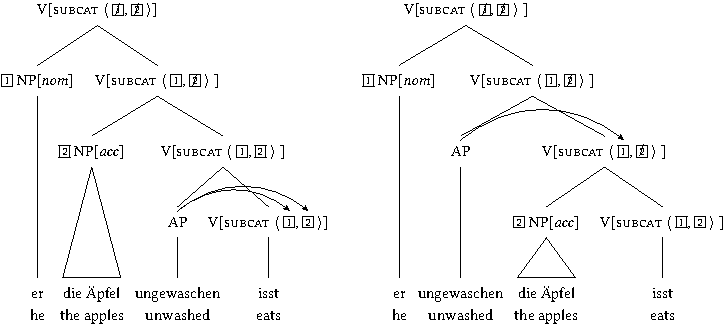
\includegraphics[width=\textwidth]{Figures/depictives-lsp-cropped.pdf}
%%  \resizebox{\linewidth}{!}{%
%% \begin{forest}
%% sm edges, for tree={l sep= 6ex}
%% [V{[\subcat \sliste{ \spirit{1}, \spirit{2} }]}
%% 	[\ibox{1} NP{[\textit{nom}]}
%% 		[er;he]]
%% 	[V{[\subcat \sliste{ \ibox{1}, \spirit{2} } ]}
%% 		[\ibox{2} NP{[\textit{acc}]}
%% 			[die Äpfel;the apples,triangle]]
%% 		[V{[\subcat \sliste{ \ibox{1}, \ibox{2} } ]}
%% 			[\subnode{ap1}{AP}
%% 				[ungewaschen;unwashed]]
%% 			[V{[\subcat \sliste{ \subnode{arg11}{\ibox{1}}, \subnode{arg12}{\ibox{2}} }]}
%% 				[isst;eats]]]]]
%% \end{forest}
%% \hspace{1em}
%% \begin{forest}
%% sm edges, for tree={l sep= 6ex}
%% [V{[\subcat \sliste{ \spirit{1}, \spirit{2} } ]}
%% 	[\ibox{1} NP{[\textit{nom}]}
%% 		[er;he]]
%% 	[V{[\subcat \sliste{ \ibox{1}, \spirit{2} } ]}
%% 		[\subnode{ap2}{AP}
%% 			[ungewaschen;unwashed]]
%% 		[V{[\subcat \sliste{ \subnode{arg21}{\ibox{1}}, \spirit{2} } ]}
%% 			[\ibox{2} NP{[\textit{acc}]}
%% 				[die Äpfel;the apples,triangle]]
%% 			[V{[\subcat \sliste{ \ibox{1}, \ibox{2} } ]}
%% 				[isst;eats]]]]]
%% \end{forest}
%% % This has to be inside of the scaling
%%     %% \begin{tikzpicture}[overlay,remember picture]
%%     %% %% this works with tikzmark
%%     %% \draw[->, bend angle=40, bend left] ($(pic cs:ap1)+(1ex,2ex)$) to($(pic cs:arg11)+(1ex,2.5ex)$);
%%     %% \draw[->, bend angle=40, bend left] ($(pic cs:ap1)+(1ex,2ex)$) to($(pic cs:arg12)+(1ex,2.5ex)$); % 1ex links, 2ex hoch
%%     %% %
%%     %% \draw[->, bend angle=40, bend left] ($(pic cs:ap2)+(1ex,2ex)$) to($(pic cs:arg21)+(1ex,2.5ex)$);
%%     %% \end{tikzpicture}
%% % somehow it stopped working
%% %% this used to work with subnode in texlive 2013 but is broken now
%% \begin{tikzpicture}[overlay,remember picture] 
%% \draw[->, bend angle=40, bend left] (ap1.north) to (arg11.north);
%% \draw[->, bend angle=40, bend left] (ap1.north) to (arg12.north); 
%% %
%% \draw[->, bend angle=40, bend left] (ap2.north) to (arg21.north);
%% \end{tikzpicture}
%}
%\hfill\mbox{}
\caption{dass er die Äpfel ungewaschen isst(\textsc{comp} 他 \defart{} 苹果 \, 没洗的 \, 吃)和dass er ungewaschen die Äpfel isst(\textsc{comp} 他 \, 没洗的 \defart{} 苹果 \, 吃)的分析}\label{anal-er-die-frau-nackt-sieht}
%\caption{Analysis of \emph{dass er die Äpfel ungewaschen isst} `that he the apples unwashed eats' and \emph{dass er ungewaschen die
%    Äpfel isst} `that he unwashed the apples eat'}\label{anal-er-die-frau-nackt-sieht}
\end{figure}%
已经实现的论元仍然在上面的结点上,但是它们已经被划掉了,因此被标注为realized(实现)。在德语中,要描述这个先行语名词的偏向可以通过假设一个限制,该限制的内容是先行语名词必须没有实现。
%Arguments that have been realized are still represented on the upper nodes, however, they are crossed-out and thereby marked as ``realized''.
%In German, this preference for the antecedent noun can be captured by assuming a restriction that states that the antecedent noun must not yet have been
%realized.

在英语\ilce{英语}{English}中,普遍假设附加语与VP组合。
%It is commonly assumed for English\il{English} that adjuncts are combined with a VP.
\eal
\ex 
\gll John [[\sub{VP} ate the apples$_i$] unwashed$_i$].\\
	John {} 吃 \defart{} 苹果 没洗的\\
\mytrans{John吃了没洗的苹果。}
%John [[\sub{VP} ate the apples$_i$] unwashed$_i$].
\ex 
\gll You can't [[\sub{VP} give them$_i$ injections] unconscious$_i$].\\
	你 能.不 {} 给 他们 注射 无意识的\\
\mytrans{你不能无意识地给他们注射。}
%You can't [[\sub{VP} give them$_i$ injections] unconscious$_i$].
\footnote{%
 \citew[\page 17]{Simpson2003a}。
}
\zl
如果有一个方法允许VP结点中动词的论元是可及的,那么即使是先行语名词在VP之后,也可以在描述性谓词和论元之间建立关系。英语与德语的不同之处在于:描述性谓词可以指向已经实现的论元,如例 (\mex{0}b)中的them,以及尚未实现的论元,如例(\mex{0}b)中的you。
%In approaches where the arguments of the verb are accessible at the VP node, it is possible to establish a relation between
%the depictive predicate and an argument although the antecedent noun is inside the VP.
%English differs from German in that depictives can refer to both realized (\emph{them} in (\mex{0}b))
%and unrealized (\emph{you} in (\mex{0}b)) arguments.

 \citet[\page 560]{Higginbotham85a}和 \citet{Winkler97a}在\gbtc 中提出了对应的非-划掉(non-cancellation)方法。在最简理论中也有类似的方法:已经检查过的特征不会被删除,但是会被标注为已经核查\citep[\page 14]{Stabler2010b}。但是,这些特征仍然被看作不可及。\label{page-non-cancellation-end}
% \citet[\page 560]{Higginbotham85a} and  \citet{Winkler97a} have proposed corresponding non-cancellation approaches in \gbt.
%There are also parallel suggestions in Minimalist theories: checked features are not deleted, but instead marked as already
%checked \citep[\page 14]{Stabler2010b}. However, these features are still viewed as inaccessible.\label{page-non-cancellation-end}

取决于投射信息的精细程度,可以在嵌套结构中看到附加语和论元以及它们的语义、句法和语义特征。在Kay和Fillmore提出的CxG变体中,所有的信息都是可及的。在LFG中,关于语法功能、格和相近特征的信息是可及的。但是,词性并不包含在f-结构中。如果词性与语法功能不是一一对应的关系,那么就不能用f-结构来限制。语音信息也不在f-结构中完全表征。如果对熟语的分析需要非局部地获取语音信息或词性信息,那么就必须明确地编码在f-结构中(关于更多熟语的问题可以参见 \citew[\page 46--50]{Bresnan82a})。
%Depending on how detailed the projected information is, it can be possible to see adjuncts and argument in embedded structures as well as their
%phonological, syntactic and semantic properties. In the CxG variant proposed by Kay and Fillmore, all information is available. In LFG,
%information about grammatical function, case and similar properties is accessible. However, the part of speech is not contained in the f-structure.
%If the part of speech does not stand in a one-to-one relation to grammatical function, it cannot be restricted using selection via f-structure.
%Nor is phonological information represented completely in the f-structure. If the analysis of idioms requires nonlocal access to phonological
%information or part of speech, then this has to be explicitly encoded in the f-structure (see  \citew[\page 46--50]{Bresnan82a} for more on idioms). 

在我采用的HPSG版本中,只有论元的信息是可以投射的。因为论元一直通过类型\type{synsem}的描述来表征,所以无法保证其语音实现的信息。但是,在结构中有子结点,仍然可能像在TAG和构式语法中制定熟语的限制条件(参见 \citew{RS2009a}对(\ref{ex-ich-glaube-mich-tritt-ein-Pferd})中horse例子的分析)。这看起来多少有点像过度描述:我们仍然投射已经实现了的论元信息(不幸的是这些也包含论元的信息等)。就这点而言,有人可能更加倾向于TAG或者LFG,因为这些理论只是对局部性进行了部分扩展:TAG使用了任意大小或者更加准确地说是所需大小的树,而LFG使用完全f-结构。但是事情好像没有这么简单:如果想在TAG中将描述性谓词与论元结合时创建与论元之间的关系,那么就需要所有可能的先行语的列表。句法因素(例如,关于与格 vs. 宾格名词短语,论元 vs.附加语,动词的并列 vs.名词的并列)在决定指称名词时非常重要,它无法通过语义关系来决定。与之相似,对于不同种类的熟语有不同的限制,并且这些都不能通过f-结构的限制来描述,因为f-结构不包括词性信息。\isce[|)]{描述性谓词}{depictive predicate}
%In the HPSG variant that I adopt, only information about arguments is projected. Since arguments are always represented by descriptions of type
%\type{synsem}, no information about their phonological realization is present. However, there are daughters in the structure so that it is still
%possible to formulate restrictions for idioms as in TAG or Construction Grammar (see  \citew{RS2009a}
%for an analysis of the `horse' example in (\ref{ex-ich-glaube-mich-tritt-ein-Pferd})).
%This may seem somewhat like overkill: although we already have the tree structure, we are still projecting information about arguments
%that have already been realized (unfortunately these also contain information about their arguments and so on). At this point, one could be inclined
%to prefer TAG or LFG since these theories only make use of one extension of locality: TAG uses trees
%of arbitrary or rather exactly the necessary size and LFG makes reference to a complete
%f-structure. However, things are not quite that simple: if one wants to create a relation to an
%argument when adjoining a depictive predicate in TAG, then one requires a list of
%possible antecedents. Syntactic factors (\eg reference to dative vs.\ accusative noun phrases, to argument vs.\ adjuncts,
%coordination of verbs vs.\ nouns) play a role in determining the referent noun, this cannot be reduced to semantic relations.
%Similarly, there are considerably different restrictions for different kinds of idioms and these cannot all be formulated in terms of restrictions
%on f-structure since f-structure does not contain information about parts of speech.\is{depictive predicate|)}

需要注意很多现象需要借助更大的单位。大部分现象可以通过中心语统制或者扩展中心语统制,但是有熟语超越句子层面。每个理论都要或多或少地解释这个问题。\isce[|)]{局部性}{locality}\isce[|)]{习语}{idiom}
%One should bear in mind that some phenomena require reference to larger portions of structure. The majority of phenomena can be treated in terms of head
%domains and extended head domains, however, there are idioms that go beyond the sentence level. Every theory has to account for this somehow.
%\is{locality|)}\is{idiom|)}



%      <!-- Local IspellDict: en_US-w_accents -->
